\let\negmedspace\undefined
\let\negthickspace\undefined
\documentclass[journal,12pt,onecolumn]{IEEEtran}
\usepackage{cite}
\usepackage{amsmath,amssymb,amsfonts,amsthm}
\usepackage{algorithmic}
\usepackage{graphicx}
\usepackage{textcomp}
\usepackage{xcolor}
\usepackage{txfonts}
\usepackage{listings}
\usepackage{enumitem}
\usepackage{circuitikz}
\usepackage{mathtools}
\usepackage{gensymb}
\usepackage{tkz-euclide} % loads  TikZ and tkz-base
\usepackage{listings}
\newtheorem{theorem}{Theorem}[section]
\newtheorem{problem}{Problem}
\newtheorem{proposition}{Proposition}[section]
\newtheorem{lemma}{Lemma}[section]
\newtheorem{corollary}[theorem]{Corollary}
\newtheorem{example}{Example}[section]
\newtheorem{definition}[problem]{Definition}
%\newtheorem{thm}{Theorem}[section] 
%\newtheorem{defn}[thm]{Definition}
%\newtheorem{algorithm}{Algorithm}[section]
%\newtheorem{cor}{Corollary}
\newcommand{\BEQA}{\begin{eqnarray}}
\newcommand{\EEQA}{\end{eqnarray}}
\newcommand{\system}[1]{\stackrel{#1}{\rightarrow}}

\newcommand{\define}{\stackrel{\triangle}{=}}
\theoremstyle{remark}
\newtheorem{rem}{Remark}
%\bibliographystyle{ieeetr}
\begin{document}
%
\providecommand{\pr}[1]{\ensuremath{\Pr\left(#1\right)}}
\providecommand{\prt}[2]{\ensuremath{p_{#1}^{\left(#2\right)} }}        % own macro for this question
\providecommand{\qfunc}[1]{\ensuremath{Q\left(#1\right)}}
\providecommand{\sbrak}[1]{\ensuremath{{}\left[#1\right]}}
\providecommand{\lsbrak}[1]{\ensuremath{{}\left[#1\right.}}
\providecommand{\rsbrak}[1]{\ensuremath{{}\left.#1\right]}}
\providecommand{\brak}[1]{\ensuremath{\left(#1\right)}}
\providecommand{\lbrak}[1]{\ensuremath{\left(#1\right.}}
\providecommand{\rbrak}[1]{\ensuremath{\left.#1\right)}}
\providecommand{\cbrak}[1]{\ensuremath{\left\{#1\right\}}}
\providecommand{\lcbrak}[1]{\ensuremath{\left\{#1\right.}}
\providecommand{\rcbrak}[1]{\ensuremath{\left.#1\right\}}}
\newcommand{\sgn}{\mathop{\mathrm{sgn}}}
\providecommand{\abs}[1]{\left\vert#1\right\vert}
\providecommand{\res}[1]{\Res\displaylimits_{#1}} 
\providecommand{\norm}[1]{\left\lVert#1\right\rVert}
%\providecommand{\norm}[1]{\lVert#1\rVert}
\providecommand{\mtx}[1]{\mathbf{#1}}
\providecommand{\mean}[1]{E\left[ #1 \right]}
\providecommand{\cond}[2]{#1\middle|#2}
\providecommand{\fourier}{\overset{\mathcal{F}}{ \rightleftharpoons}}
\newenvironment{amatrix}[1]{%
  \left(\begin{array}{@{}*{#1}{c}|c@{}}
}{%
  \end{array}\right)
}
%\providecommand{\hilbert}{\overset{\mathcal{H}}{ \rightleftharpoons}}
%\providecommand{\system}{\overset{\mathcal{H}}{ \longleftrightarrow}}
	%\newcommand{\solution}[2]{\textbf{Solution:}{#1}}
\newcommand{\solution}{\noindent \textbf{Solution: }}
\newcommand{\cosec}{\,\text{cosec}\,}
\providecommand{\dec}[2]{\ensuremath{\overset{#1}{\underset{#2}{\gtrless}}}}
\newcommand{\myvec}[1]{\ensuremath{\begin{pmatrix}#1\end{pmatrix}}}
\newcommand{\mydet}[1]{\ensuremath{\begin{vmatrix}#1\end{vmatrix}}}
\newcommand{\myaugvec}[2]{\ensuremath{\begin{amatrix}{#1}#2\end{amatrix}}}
\providecommand{\rank}{\text{rank}}
\providecommand{\pr}[1]{\ensuremath{\Pr\left(#1\right)}}
\providecommand{\qfunc}[1]{\ensuremath{Q\left(#1\right)}}
	\newcommand*{\permcomb}[4][0mu]{{{}^{#3}\mkern#1#2_{#4}}}
\newcommand*{\perm}[1][-3mu]{\permcomb[#1]{P}}
\newcommand*{\comb}[1][-1mu]{\permcomb[#1]{C}}
\providecommand{\qfunc}[1]{\ensuremath{Q\left(#1\right)}}
\providecommand{\gauss}[2]{\mathcal{N}\ensuremath{\left(#1,#2\right)}}
\providecommand{\diff}[2]{\ensuremath{\frac{d{#1}}{d{#2}}}}
\providecommand{\myceil}[1]{\left \lceil #1 \right \rceil }
\newcommand\figref{Fig.~\ref}
\newcommand\tabref{Table~\ref}
\newcommand{\sinc}{\,\text{sinc}\,}
\newcommand{\rect}{\,\text{rect}\,}
%%
%	%\newcommand{\solution}[2]{\textbf{Solution:}{#1}}
%\newcommand{\solution}{\noindent \textbf{Solution: }}
%\newcommand{\cosec}{\,\text{cosec}\,}
%\numberwithin{equation}{section}
%\numberwithin{equation}{subsection}
%\numberwithin{problem}{section}
%\numberwithin{definition}{section}
%\makeatletter
%\@addtoreset{figure}{problem}
%\makeatother

%\let\StandardTheFigure\thefigure
\let\vec\mathbf

\bibliographystyle{IEEEtran}





\bigskip



\title{Analog Assignment}
\author{Karyampudi Meghana Sai\\ EE23BTECH11031}
\maketitle

In Exercises 7.3 and 7.4,what is the net power absorbed by each circuit over a complete cycle. Explain your answer.\\
\solution
(a) In Exercise 7.3 :
\begin{figure}[h]
	\centering
	\begin{circuitikz}
    % Draw the components and connect them
    \draw (0,2) to[L, l=$44\,mH$] (4,2)
    (0,0) to[V, v=$220\,V$, f=$50\,Hz$] (4,0)
    (0,2) -- (0,0)
    (4,2) -- (4,0);
\end{circuitikz}

	\caption{Inductive Circuit}
	\label{}
\end{figure}
\begin{table}[h]
 	\centering
 	\resizebox{6 cm}{!}{
 		\begin{tabular}{|c|c|c|}
	\hline
	\textbf{Symbol} & \textbf{Value} &
	\textbf{Description}\\[6pt]
	\hline
	$L$ &  $44mH$ & Inductance\\[6pt]
	\hline 
	$V_{rms}$ & $220\, V$ & Voltage\\[6pt]
	\hline
	$f$ & $50\, {Hz}$ & Frequency\\[6pt]
	\hline
	$\omega$ & $2\pi f=100\pi$ & Angular Frequency\\[6pt]
	\hline
	$\phi$ & $?$ & Phase difference between current and voltage\\[6pt]
	\hline
	$I_ \text{rms}$ & $15.92\, A$ & rms value of current\\
	\hline
\end{tabular}

 	}
 	\vspace{6 pt}
 	\caption{Input Parameters}
 	\label{table:12.7.5table1} 
 \end{table} 
 \begin{figure}[h]
	\centering
	\begin{circuitikz}
    % Draw the components and connect them
    \draw (0,0) -- (1,0);
    \draw (1,0) to [L, l = $sL$] (2,0);
    \draw (2,0) -- (3,0);
    \draw (3,0) -- (3,-2);
    \draw (0,0) -- (0,-1);
    \draw[->] (0,-1) node[left] {$I(s)$} -- (0,-1);
    \draw (0,-1) -- (0,-2);
    \draw (0,-2) -- (1,-2);
    \draw (1,-2) to [sV, l = $V(s)$] (2,-2);
    \draw (2,-2) -- (3,-2);
\end{circuitikz}

	\caption{s domain Circuit}
	\label{}
\end{figure}
\begin{align}
        V(s) = I(s)\brak{sL} \label{eq:12.7.5eq1}
 \end{align}
\begin{align}
    I(s) &= \dfrac{V(s)}{\brak{sL}}\label{eq:12.7.5eq2}\\ 
    H(s) &= \dfrac{V(s)}{I(s)}\label{eq:12.7.5eq3}\\
	H(s) &= sL\label{eq:12.7.5eq4}
\end{align}

Substituting $s$ with j $\omega$ :
\begin{equation}
	H(j\omega) = j\omega L\label{eq:12.7.5eq5}
\end{equation}
Average power absorbed by the inductor in the circuit is given by:
\begin{align}
	P=VIcos(\phi) \label{eq:12.7.5eq6}
\end{align}
For an inductor the phase angle is:
\begin{align}
	\phi &= -\frac{\pi}{2}\label{eq:12.7.5eq7}\\
	cos(\phi) &= 0\label{eq:12.7.5eq8}\\
	P_L &= 0\label{eq:12.7.5eq9}
\end{align}	
\begin{figure}[h!]
  \centering
  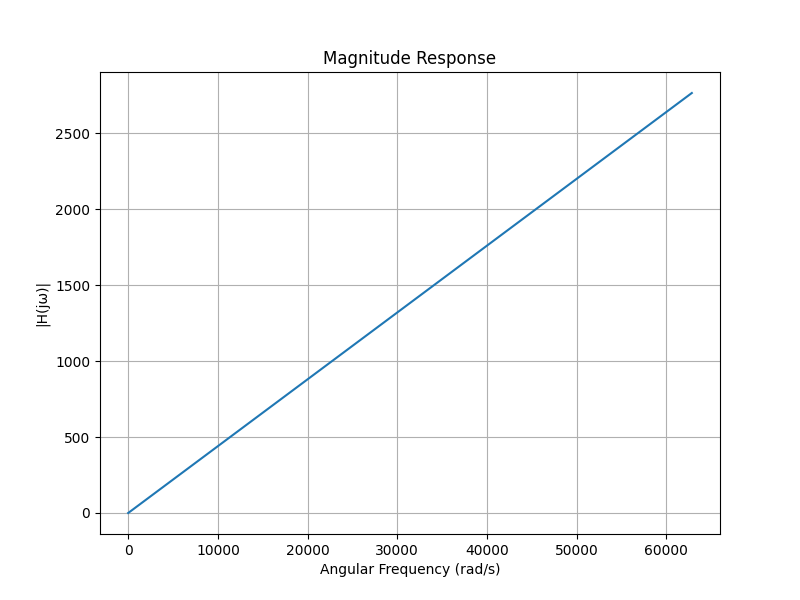
\includegraphics[width=\columnwidth]{figs/plot1.png}
  \caption{Plot of equation\eqref{eq:12.7.5eq5}}
  \label{}
\end{figure}
(b) In Exercise 7.4 :
\begin{figure}[h]
	\centering
	\begin{circuitikz}
    % Draw the components and connect them
    \draw (0,2) to[C, l=$60\,\mu F$] (4,2)
    (0,0) to[V, v=$110\,V$, f=$60\,Hz$] (4,0)
    (0,2) -- (0,0)
    (4,2) -- (4,0);
\end{circuitikz}

	\caption{Capacitive Circuit}
	\label{}
\end{figure}
\begin{table}[h]
 	\centering
 	\resizebox{6 cm}{!}{
 		\begin{tabular}{|c|c|c|}
	\hline
	\textbf{Symbol} & \textbf{Value} &
	\textbf{Description}\\[6pt]
	\hline
	$C$ &  $60\, \mu F$ & Capacitance \\[6pt]
	\hline
	$V_{rms}$ & $110\, V$ & Voltage\\[6pt]
	\hline
	$f$ & $60\, {Hz}$ & Frequency\\[6pt]
	\hline
	$\omega$ & $2\pi f=120\pi$ & Angular Frequency\\[6pt]
	\hline
	$\phi$ & $?$ & Phase difference between current and voltage\\[6pt]
	\hline
	$I_ \text{rms}$ & $2.49\, A$ & rms value of current\\
	\hline
\end{tabular}

 	}
 	\vspace{6 pt}
 	\caption{Input Parameters}
 	\label{} 
 \end{table} 
\begin{figure}[h!]
	\centering
	\begin{circuitikz}
    % Draw the components and connect them
    \draw (0,0) -- (1,0);
    \draw (1,0) to [C, l = $\frac{1}{sC}$] (2,0);
    \draw (2,0) -- (3,0);
    \draw (3,0) -- (3,-2);
    \draw (0,0) -- (0,-1);
    \draw[->] (0,-1) node[left] {$I(s)$} -- (0,-1);
    \draw (0,-1) -- (0,-2);
    \draw (0,-2) -- (1,-2);
    \draw (1,-2) to [sV, l = $V(s)$] (2,-2);
    \draw (2,-2) -- (3,-2);
\end{circuitikz}

	\caption{s domain Circuit}
	\label{}
\end{figure}
\begin{align}
        V(s) = I(s)\brak{\frac{1}{sC}}\label{eq:12.7.5eq10}
 \end{align}
\begin{align}
    I(s) &= \dfrac{V(s)}{\brak{\frac{1}{sC}}}\label{eq:12.7.5eq11}\\ 
    H(s) &= \dfrac{V(s)}{I(s)}\label{eq:12.7.5eq12}\\
	H(s) &= \frac{1}{sC}\label{eq:12.7.5eq13}
\end{align}
Substituting $s$ with j $\omega$:
\begin{equation}
	H(j\omega) = \frac{1}{j\omega C }\label{eq:12.7.5eq14}
\end{equation}
Average power absorbed by the capacitor in the circuit is given by:
\begin{align}
	P=VIcos(\phi) \label{eq:12.7.5eq15}
\end{align}
For an capacitor the phase angle is:
\begin{align}
	\phi &= \frac{\pi}{2}\label{eq:12.7.5eq16}\\
	cos(\phi) &= 0\label{eq:12.7.5eq17}\\
	P_C &= 0\label{eq:12.7.5eq18}
\end{align}
\begin{figure}[h!]
  \centering
  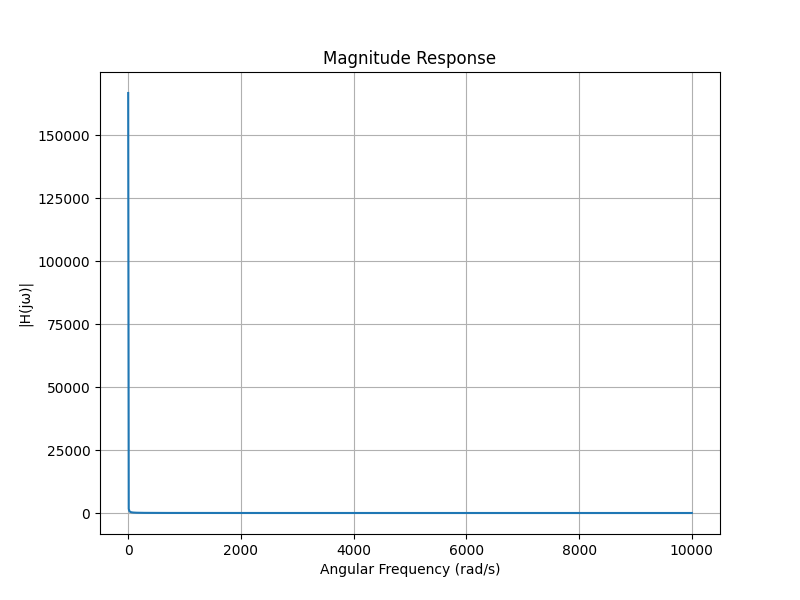
\includegraphics[width=\columnwidth]{figs/plot2.png}
  \caption{Plot of equation\eqref{eq:12.7.5eq14}}
  \label{}
\end{figure}	
\end{document}
